\documentclass[12pt]{article}
\usepackage{amsfonts, epsfig}

\usepackage{graphicx}
\usepackage{fancyhdr}
\usepackage{amsmath}
\pagestyle{fancy}
\usepackage{xcolor}
\usepackage[latin9]{inputenc}
\usepackage[T1]{fontenc}
\lfoot{\texttt{github.com/COMS30127}}
\lhead{Computational Neuroscience - Coursework 3 - IandF/STDP (resit)}
\rhead{\thepage}
\cfoot{}
\begin{document}

\section*{Coursework 3 (resit)}
This coursework has two parts: part A on the integrate-and-fire neuron model (worth 25\% of the coursework grade) and part B on spike-timing-dependent-plasticity (worth 75\% of the coursework grade). COMS30127 marks add up nicely to 100, but for COMSM2127 the marks add up to 135 -- don't worry we will normalise these (within each part) after marking.

Write a brief report, around five or six or seven pages,
including the figures and the comments specified. No need to be verbose, just say what you are asked to say. We will take a dim view of super-narrow margins or tiny fonts. Submit it in the pdf format
together with the Python or Julia or MATLAB code by the deadline. Submit the report as pdf; make
sure to set the size of the graphs in your plotting program, not by
shrinking the graph to fit in the report, this makes the figure
legends and axis numbers tiny and is super annoying. You don't have to
plot in Python or Julia or MATLAB, it is fine to output a data file and plot
using gnuplot or whatever. All plots should have clear x- and y-axis labels, and units. Four marks will be docked for every plot that has missing or unclear labels.

\textcolor{black}{To help you decide which results to include in your
report, I will encode meaning in my text colour and formatting. }\textcolor{magenta}{If
a sentence is coloured magenta, I expect to see a written response}.
\emph{For sentences formatted with italics I expect to see a plot}.

Submit your report on Blackboard. The deadline is 1pm on Monday 18th August 2020.

\section*{Part A: Integrate-and-fire neurons (25\% of coursework grade)}

\subsection*{Question 1 [10 marks]}

Simulate an integrate and fire model with the following parameters for
1 s: $\tau_m = 10 $ms, $E_L = V_{rest} = -70$ mV, $V_{th} = -54$ mV, $R_m= 8$
M$\Omega$, $I_e = 2.1 $ nA. Here $E_L$ is the leak potential, $V_{rest}$ is the reset voltage,
$V_{th}$ is the threshold, $R_m$ is the membrane resistance, that is one
over the conductance, and $\tau_m$ is the membrane time constant. Use Euler's method with timestep $\delta t
= 0.25$ ms to solve the differential equations numerically. Make sure to use the differential equations, do not just plot the analytical solution for V(t) given in the lectures/notes -- this will be useless for later questions anyway.

\emph{Plot the voltage as a function of time}. For simplicity assume that the
neuron does not have a refractory period after producing a spike. You
do not need to plot spikes -- once membrane potential exceeds
threshold, simply set the membrane potential to $V_{rest}$. To keep track of the units I recommend converting everything to S.I. units inside your simulation code -- you don't have to do this but it often makes things easier.

\subsection*{Question 2 [15 marks]}

Simulate two neurons which have synaptic connections between
  each other, that is the first neuron projects to the second, and the
  second neuron projects to the first. Both model neurons should have
  the same parameters: $\tau_m = 20$ ms, $E_L = -70$ mV, $V_{rest} = -80$ mV,
  $V_{th} = -54$ mV, $R_mI_e = 18$ mV, and their synapses should also have
  the same parameters: $R_m \bar{g}_s = 0.15$, $\Delta s = 0.5$, $\tau_s= 10$
  ms; don't get confused by being given $R_m\bar{g}_s$ rather than
  $\bar{g}_s$ on its own, to get $\tau_m$ rather than the capacitance
  on the left hand side of the integrate and fire equation everything
  is multiplied by $R_m$. For simplicity take the synaptic conductance
\begin{equation}
g_s=\bar{g}_s s
\end{equation}
to satisfy
\begin{equation}
\tau_s\frac{ds}{dt}=-s
\end{equation}
with a spike arriving causing $s$ to increase instantaneously by an amount $\Delta s$. This is
equivalent to the simplest synapse model in lecture 16. Simulate two
cases: a) assuming that the synapses are excitatory with $E_s = 0$ mV,
and b) assuming that the synapses are inhibitory with $E_s = -80$
mV. For each simulation set the initial membrane potentials of the
neurons $V$ to different values chosen randomly from between $V_{rest}$ and
$V_{th}$ and simulate 1 s of activity. \emph{For each case plot the voltages of
the two neurons on the same graph (with different colours).}  \textcolor{magenta}{Comment on what is happening in each case. Offer an explanation for what you observe.}

\subsection*{COMSM2127 [15 marks]}

This question uses parameters from Q1 above.

\begin{enumerate}

\item \textcolor{magenta}{Compute analytically} the minimum current $I_e$ required for the
  neuron with the above parameters to produce an action
  potential.

\item Simulate the neuron for 1 s for the input current with amplitude
  $I_e$ which is 0.1 [nA] lower than the minimum current computed
  above, and \emph{plot the voltage as a functions of time}.

\item Simulate the neuron for 1s for currents ranging from 1 [nA] to 5
  [nA] in steps of 0.1 [nA]. For each amplitude of current count the
  number of spikes produced, that is the firing rate. \emph{Plot the firing
  rate as the function of the input current.} 

\end{enumerate}

\section*{Part B: STDP (75\% of coursework grade)}
Now make a new simulation of a single leaky-integrate-and-fire neuron (you can reuse appropriate bits of your code from Part A). Set the resting potential $V_{rest}= E_L = -65$ mV,
spike threshold $V_{th}=-50$ mV, reset voltage $V_{reset}=V_{rest}=-65$
mV, a passive membrane leak conductance that gives an input resistance
of $R_{m}=100$ M$\Omega$, and $\tau_{m}=10$
ms. Note that these values are different to those used above in Part A. Don't include a background input current, $I_e=0$. Add $N=40$ incoming synapses (just model the synaptic responses to spike trains, do not
explicitly simulate the somatic voltages of these presynaptic neurons).
Model all synapses as a conductance-based, following a single-exponential
timecourse with decay time constant $\tau_{s}=2$ ms, the initial
peak conductances (strengths) all $\bar{g}_i = 4$ nanoSiemens for all synapses, $E_s=0$, and $\Delta s=0.5$. Let $s_i (t=0)=0$ for all 40 synapses. You should have 40 different $s_i$ variables and 40 different $\bar{g}_i$ variables in total, since you have 40 synapses. It's probably easier to store them all in arrays and update them together, rather than code each one by hand. Use the Euler method to solve the system of ODEs (40 $s$ variables plus 1 voltage variable), with a simulation timestep $\delta t=0.25$ milliseconds.

Simulate each input spike train as an independent homogeneous Poisson
process with the same average firing rate $\langle r\rangle$. A homogeneous
Poisson process implies that average firing rate $\langle r\rangle$
is fixed in time, but that the spikes themselves arrive randomly.
Initially set $\langle r\rangle=15$ Hz. There are multiple ways to
simulate Poisson spike trains. In principle you could use the function from the previous coursework 2 to pre-compute poisson spike times, but for the current exercise it will be easier to do it online during the simulation. One simple method is
to draw a random number on the unit interval for each synapse at every
timestep, then if that number is less than $\langle r\rangle\delta t$,
assume a spike has occurred at that synapse. This method is valid as
long as $\langle r\rangle\delta t\ll1$.

\subsection*{Question 1 [15 marks]}
Initially set all the synapses at the same strength, equal to the maximal conductance (4 nS). Simulating your model at this stage should result in the neuron firing irregularly at a rate of roughly 20 Hz. \emph{Plot the neuron's voltage for one second of simulation time.}


\subsection*{Question 2 [20 marks]}
Now add STDP to the model using the following basic rule. First, let's denote
a presynaptic spike time as $t_{pre}$, postsynaptic spike time as
$t_{post}$, and the difference in pre-post spike times as $\Delta t=t_{post}-t_{pre}$
(so that pre-before-post timings are positive, while post-before-pre
timings are negative). Now the rule for changing the synaptic conductance
$\bar{g}_{syn}\rightarrow\bar{g}_{syn}+f(\Delta t$), with 
\[
f(\Delta t)=
\begin{cases} A_{+}\exp(-|\Delta t|/\tau_{+})  \quad  &{\rm if} \quad \Delta t>0 \cr
-A_{-}\exp(-|\Delta t|/\tau_{-}) \quad  &{\rm if}\quad \Delta t\leq0 \cr
\end{cases}
%A_{+}\exp(-|\Delta t|/\tau_{+}) \quad {\rm if} \quad\Delta t>0\\
%-A_{-}\exp(-|\Delta t|/\tau_{-}) & {\rm if}\quad\Delta t\leq0
\]

\begin{figure}[h!]
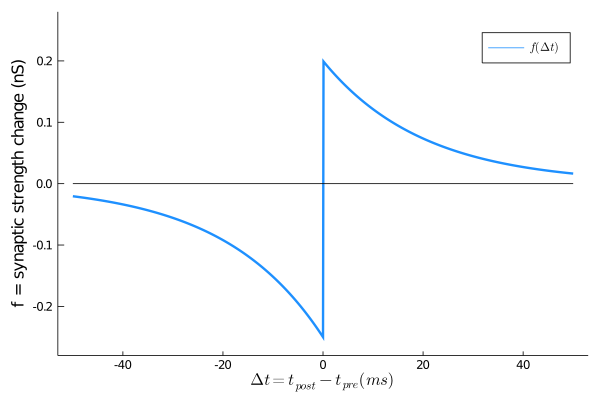
\includegraphics[width=0.8\textwidth]{stdp.png}
\end{figure}

Initially set the four STDP model parameters as: $A_{+}=0.2$ nS ,
$A_{-}=0.25$ nS, $\tau_{+}=20$ ms, $\tau_{-}=20$ ms. The synaptic
strength updates should follow the `nearest neighbour' principle:
only include the most recent pre and post spikes in your weight update
calculations. Finally, impose hard limits on the synaptic strengths
during the entire simulations: if an update would make a synaptic
weight negative, set it to zero; if an update would make the synaptic
weight greater than 4 nS, cap it at exactly 4 nS instead.

One convenient trick that simplifies programming is to note that potentiation happens at all synapses whenever a post-synaptic spike occurs, whereas depression happens at the synapses that receive a pre-synaptic spike.

Include a flag in your code that lets you switch the simulation mode
from having STDP `on' or `off'. STDP `on' mode means that every
spike (pre and post) triggers changes in the maximum conductances
of the activated synapses according to the above rule, while STDP
`off' mode means that synaptic strengths are fixed and remain stuck
at the same values throughout the simulation.

% Finally, because these simulations are stochastic, any numbers that
% you measure will likely change a little bit each time you run the
% simulation. Hence any values you include in your report should come
% from averages over multiple realisations (repeats) of the simulations.

Now set the STDP flag to `on', initialise all the synaptic strengths to 4 nS and set the input firing rates $\langle r\rangle=15$
Hz. Run the simulation for 300 s of biological time. \textcolor{magenta}{What qualitative shape does the synaptic strength distribution converge towards at the end of the simulation time?} (You might need to run the simulation a few times to see the pattern).
\emph{Plot a histogram of the steady-state synaptic weights after
one run of the simulation. Also plot the average firing rate of the
postsynaptic neuron as a function of time across the entire
300 second simulation (taking 10-second time bins).}

\subsection*{Question 3 [20 marks]} Vary the input firing rates from 10 Hz up to 20 Hz,
both for a set of simulations with STDP switched on and for a set
of simulations with STDP switched off. For both cases initialise the synaptic strengths at their maximum value, 4 nS. \textcolor{magenta}{How does
the steady-state output firing rate depend on the input firing rates
in both cases?} \emph{Plot the mean output firing rate as a function
of the input firing rates for both cases. Plot the steady-state synaptic strength
distribution for $\langle r\rangle=10$ Hz and $\langle r\rangle=20$
Hz for the `STDP on' case.} \textcolor{magenta}{Give an explanation of what is happening and why you think it makes sense.}

\subsection*{Question 4 [20 marks]} Now split the 40 input synapses into two equal sized groups ($N_{1}=20$, $N_{2}=20$). Set the first input group's spike trains to have firing rate $\langle r_1\rangle  = 10$ Hz and the firing rate of the second group's spike trains to $\langle r_2\rangle =20$ Hz. \textcolor{magenta}{Report the mean steady-state synaptic strength from each group of inputs.} Note that the mean total rate of input spikes to the neuron is $(10+20)/2 = 15$ Hz. \textcolor{magenta}{How do these mean synaptic strength values compare with the synaptic strength you found for the $\langle r\rangle=15$ Hz case from Q3? Give an explanation for these results.}


\subsection*{COMSM2127 [20 marks]} Now fix $\langle r_1\rangle =15$ Hz and run the simulation multiple times varying $\langle r_2\rangle$ between 10 Hz and 20 Hz. \emph{Plot the mean steady--state synaptic strength of each group of inputs as a function of $r_2$.} \emph{Plot example histograms of steady-state synaptic strengths for each group of synapses from simulations where $\langle r_2\rangle=10$ Hz and for $\langle r_2\rangle=20$ Hz.}


\end{document}
